\documentclass[14pt,a4paper]{extarticle}

\usepackage[utf8]{inputenc}
\usepackage[T2A]{fontenc}
\usepackage[russian]{babel}
\usepackage{pscyr}

\usepackage{geometry}
\geometry{left=30mm,right=15mm,top=20mm,bottom=20mm}

\usepackage{setspace}
\singlespacing
\renewcommand{\baselinestretch}{1.0}
\setlength{\parskip}{0pt}

\usepackage{indentfirst}
\setlength{\parindent}{1.25cm}

\usepackage{amsmath,amssymb}
\usepackage{graphicx}
\usepackage{float}
\usepackage{caption}
\usepackage{enumitem}
\usepackage{booktabs}
\usepackage{tabularx}

\usepackage{titlesec}

\titleformat{\section}
  {\normalfont\fontsize{14}{18}\bfseries\filright}
  {\thesection}{1em}{}
\titlespacing*{\section}{1.25cm}{14pt}{14pt}

\titleformat{\subsection}
  {\normalfont\fontsize{14}{18}\bfseries\filright}
  {\thesubsection}{1em}{}
\titlespacing*{\subsection}{1.25cm}{14pt}{14pt}

\usepackage{tocloft}
\renewcommand{\cfttoctitlefont}{\hfill\fontsize{14}{18}\selectfont\bfseries}
\renewcommand{\cftaftertoctitle}{\hfill}
\renewcommand{\cftsecfont}{\normalfont}
\renewcommand{\cftsecpagefont}{\normalfont}
\renewcommand{\cftsubsecfont}{\normalfont}
\renewcommand{\cftsubsecpagefont}{\normalfont}
\renewcommand{\cftdotsep}{1}
\renewcommand{\cftsecleader}{\cftdotfill{\cftdotsep}}

\usepackage{listings}
\lstset{
  basicstyle=\ttfamily\small,
  frame=single,
  breaklines=true,
  showstringspaces=false,
  inputencoding=utf8,
  extendedchars=true,
  literate={а}{{\cyra}}1 {б}{{\cyrb}}1 {в}{{\cyrv}}1 {г}{{\cyrg}}1
           {д}{{\cyrd}}1 {е}{{\cyre}}1 {ж}{{\cyrzh}}1 {з}{{\cyrz}}1
           {и}{{\cyri}}1 {й}{{\cyrishrt}}1 {к}{{\cyrk}}1 {л}{{\cyrl}}1
           {м}{{\cyrm}}1 {н}{{\cyrn}}1 {о}{{\cyro}}1 {п}{{\cyrp}}1
           {р}{{\cyrr}}1 {с}{{\cyrs}}1 {т}{{\cyrt}}1 {у}{{\cyru}}1
           {ф}{{\cyrf}}1 {х}{{\cyrh}}1 {ц}{{\cyrc}}1 {ч}{{\cyrch}}1
           {ш}{{\cyrsh}}1 {щ}{{\cyrshch}}1 {ъ}{{\cyrhrdsn}}1 {ы}{{\cyrery}}1
           {ь}{{\cyrsftsn}}1 {э}{{\cyrerev}}1 {ю}{{\cyryu}}1 {я}{{\cyrya}}1
           {А}{{\CYRA}}1 {Б}{{\CYRB}}1 {В}{{\CYRV}}1 {Г}{{\CYRG}}1
           {Д}{{\CYRD}}1 {Е}{{\CYRE}}1 {Ж}{{\CYRZH}}1 {З}{{\CYRZ}}1
           {И}{{\CYRI}}1 {Й}{{\CYRISHRT}}1 {К}{{\CYRK}}1 {Л}{{\CYRL}}1
           {М}{{\CYRM}}1 {Н}{{\CYRN}}1 {О}{{\CYRO}}1 {П}{{\CYRP}}1
           {Р}{{\CYRR}}1 {С}{{\CYRS}}1 {Т}{{\CYRT}}1 {У}{{\CYRU}}1
           {Ф}{{\CYRF}}1 {Х}{{\CYRH}}1 {Ц}{{\CYRC}}1 {Ч}{{\CYRCH}}1
           {Ш}{{\CYRSH}}1 {Щ}{{\CYRSHCH}}1 {Ъ}{{\CYRHRDSN}}1 {Ы}{{\CYRERY}}1
           {Ь}{{\CYRSFTSN}}1 {Э}{{\CYREREV}}1 {Ю}{{\CYRYU}}1 {Я}{{\CYRYA}}1
           {ё}{{\cyryo}}1 {Ё}{{\CYRYO}}1,
  numbers=left,
  numberstyle=\tiny,
  tabsize=2,
  language=R
}

\usepackage{hyperref}
\hypersetup{
    colorlinks=true,
    linkcolor=black,
    urlcolor=blue,
    citecolor=black,
}

\usepackage{fancyhdr}
\pagestyle{fancy}
\fancyhf{}
\fancyfoot[R]{\thepage}
\renewcommand{\headrulewidth}{0pt}

\begin{document}

% =========================================================
% ТИТУЛЬНЫЙ ЛИСТ
% =========================================================
\thispagestyle{empty}
\begin{center}
МИНИСТЕРСТВО ОБРАЗОВАНИЯ РЕСПУБЛИКИ БЕЛАРУСЬ

\vspace{0.5em}

Учреждение образования

\textbf{<<Белорусский государственный университет\\информатики и радиоэлектроники>>}

\vspace{2em}

Факультет компьютерных систем и сетей

\vspace{0.5em}

Кафедра программного обеспечения информационных технологий
\end{center}

\vspace{4em}

\begin{center}
\textbf{ОТЧЁТ}

по лабораторной работе №2

\vspace{0.5em}

по дисциплине <<Стили и методы программирования>>

\vspace{1em}

\textbf{Тема: <<Основы анализа и визуализации данных на языке R>>}
\end{center}

\vspace{6em}

\begin{flushright}
\begin{minipage}{0.5\textwidth}
\textbf{Выполнил:}\\
Лебедевич Артем Владимирович\\
магистрант факультета\\
компьютерных систем и сетей\\
группы 556301

\vspace{1em}

\textbf{Преподаватель:}\\
Парамонов Антон Иванович\\
кандидат технических наук, доцент\\
заведующий кафедрой информационных\\
систем и технологий ИТТ БГУИР
\end{minipage}
\end{flushright}

\vfill

\begin{center}
Минск, 2026
\end{center}

\newpage

% =========================================================
% СОДЕРЖАНИЕ
% =========================================================
\tableofcontents
\newpage

% =========================================================
% ВВЕДЕНИЕ
% =========================================================
\addcontentsline{toc}{section}{Введение}
\section*{ВВЕДЕНИЕ}

Анализ данных является одной из ключевых задач в современной информатике и науке о данных. Язык R предоставляет мощные средства для загрузки данных из внешних источников, их статистической обработки и визуализации с помощью как встроенных средств, так и внешних библиотек.

Целью данной лабораторной работы является освоение методов подключения к удалённым источникам данных, загрузки и сохранения выборок, проведения статистического анализа (кластеризации) и построения информативных графиков с использованием библиотек языка R.

\newpage

% =========================================================
% РАЗДЕЛ 1
% =========================================================
\section{ИСТОЧНИКИ ДАННЫХ И ВЫБОРКА}

В качестве удалённого ресурса используется открытый API-сервис JSONPlaceholder (\url{https://jsonplaceholder.typicode.com}), предоставляющий тестовые данные в формате JSON для разработки и прототипирования.

Из сервиса загружается выборка данных о пользователях (эндпоинт \texttt{/users}), содержащая 10 записей со следующими полями:
\begin{itemize}[nosep]
  \item \texttt{id}~-- идентификатор пользователя;
  \item \texttt{name}~-- имя пользователя;
  \item \texttt{username}~-- логин;
  \item \texttt{email}~-- электронная почта;
  \item \texttt{address}~-- адрес (включая географические координаты \texttt{geo.lat}, \texttt{geo.lng});
  \item \texttt{phone}, \texttt{website}, \texttt{company}~-- контактные данные и информация о компании.
\end{itemize}

Данные загружаются через HTTP GET-запрос и сохраняются в локальный файл \texttt{users\_data.csv} в формате CSV.

\newpage

% =========================================================
% РАЗДЕЛ 2
% =========================================================
\section{ОПИСАНИЕ ИНДИВИДУАЛЬНОГО ЗАДАНИЯ И АЛГОРИТМ РЕШЕНИЯ}

Индивидуальное задание заключается в кластеризации пользователей по их географическому расположению с использованием метода k-средних.

Общий алгоритм решения:

1 Подключение к удалённому API и загрузка данных в формате JSON (Скрипт~1).

2 Парсинг JSON-ответа и сохранение данных в локальный CSV-файл.

3 Загрузка данных из локального CSV-файла в рабочую среду R (Скрипт~2).

4 Извлечение числовых признаков~-- географических координат (широта и долгота).

5 Применение алгоритма кластеризации k-means с числом кластеров $k = 3$.

6 Визуализация результатов кластеризации на диаграмме рассеяния.

7 Построение столбиковой диаграммы распределения пользователей по кластерам.

8 Сохранение графических результатов в файлы формата PNG.

\newpage

% =========================================================
% РАЗДЕЛ 3
% =========================================================
\section{ИСПОЛЬЗУЕМЫЕ БИБЛИОТЕКИ R}

В таблице~\ref{tab:libs} приведён перечень библиотек, использованных при выполнении задания.

\begin{table}[H]
\caption{Библиотеки R, использованные в проекте}
\label{tab:libs}
\begin{tabularx}{\textwidth}{|l|X|}
\hline
\textbf{Библиотека} & \textbf{Назначение} \\
\hline
httr & Выполнение HTTP-запросов (GET, POST и др.) для подключения к удалённым ресурсам \\
\hline
jsonlite & Парсинг JSON-данных, преобразование между JSON и data.frame \\
\hline
ggplot2 & Построение графиков высокого качества на основе грамматики графики \\
\hline
dplyr & Манипуляция данными: фильтрация, выборка столбцов, группировка \\
\hline
corrplot & Визуализация корреляционных матриц \\
\hline
cluster & Методы кластерного анализа \\
\hline
\end{tabularx}
\end{table}

\newpage

% =========================================================
% РАЗДЕЛ 4
% =========================================================
\section{ФРАГМЕНТЫ КОДА}

\subsection{Скрипт 1~-- загрузка данных с удалённого ресурса}

\begin{lstlisting}[caption={Скрипт lab2\_script1.R}, label=lst:script1]
library(httr)
library(jsonlite)

# Подключение к удаленному ресурсу
url <- "https://jsonplaceholder.typicode.com/users"
response <- GET(url)

if (status_code(response) == 200) {
  cat("Подключение успешно. Код:", status_code(response), "\n")
} else {
  stop("Ошибка подключения: ", status_code(response))
}

# Выгрузка и сохранение данных
users_json <- content(response, as = "text", encoding = "UTF-8")
users_data <- fromJSON(users_json, flatten = TRUE)

cat("Загружено записей:", nrow(users_data), "\n")

write.csv(users_data, file = "users_data.csv",
          row.names = FALSE, fileEncoding = "UTF-8")
cat("Данные сохранены в users_data.csv\n")
\end{lstlisting}

\newpage

\subsection{Скрипт 2~-- анализ и визуализация данных}

\begin{lstlisting}[caption={Скрипт lab2\_script2.R}, label=lst:script2]
library(ggplot2)
library(dplyr)
library(cluster)

# Загрузка из локального файла
users_data <- read.csv("users_data.csv", fileEncoding = "UTF-8")

# Подготовка числовых данных
numeric_data <- users_data %>%
  select(address.geo.lat, address.geo.lng) %>%
  mutate(
    address.geo.lat = as.numeric(address.geo.lat),
    address.geo.lng = as.numeric(address.geo.lng)
  )

# Кластерный анализ k-means
set.seed(42)
kmeans_result <- kmeans(numeric_data, centers = 3, nstart = 25)
users_data$cluster <- as.factor(kmeans_result$cluster)

# Диаграмма рассеяния с кластерами
p1 <- ggplot(users_data,
       aes(x = as.numeric(address.geo.lng),
           y = as.numeric(address.geo.lat),
           color = cluster)) +
  geom_point(size = 4) +
  geom_text(aes(label = name), vjust = -1, size = 3) +
  labs(title = "Кластеризация по геолокации",
       x = "Долгота", y = "Широта",
       color = "Кластер") +
  theme_minimal()
print(p1)

# Столбиковая диаграмма
p2 <- ggplot(users_data, aes(x = cluster, fill = cluster)) +
  geom_bar() +
  labs(title = "Распределение по кластерам",
       x = "Кластер", y = "Количество") +
  theme_minimal()
print(p2)

# Сохранение графиков
ggsave("cluster_scatter.png", plot = p1,
       width = 10, height = 7, dpi = 150)
ggsave("cluster_bar.png", plot = p2,
       width = 8, height = 6, dpi = 150)
\end{lstlisting}

\newpage

% =========================================================
% РАЗДЕЛ 5
% =========================================================
\section{ГРАФИЧЕСКИЕ РЕЗУЛЬТАТЫ РАБОТЫ СКРИПТА}

В данном разделе представлены графические результаты работы скрипта.

\begin{figure}[H]
  \centering
  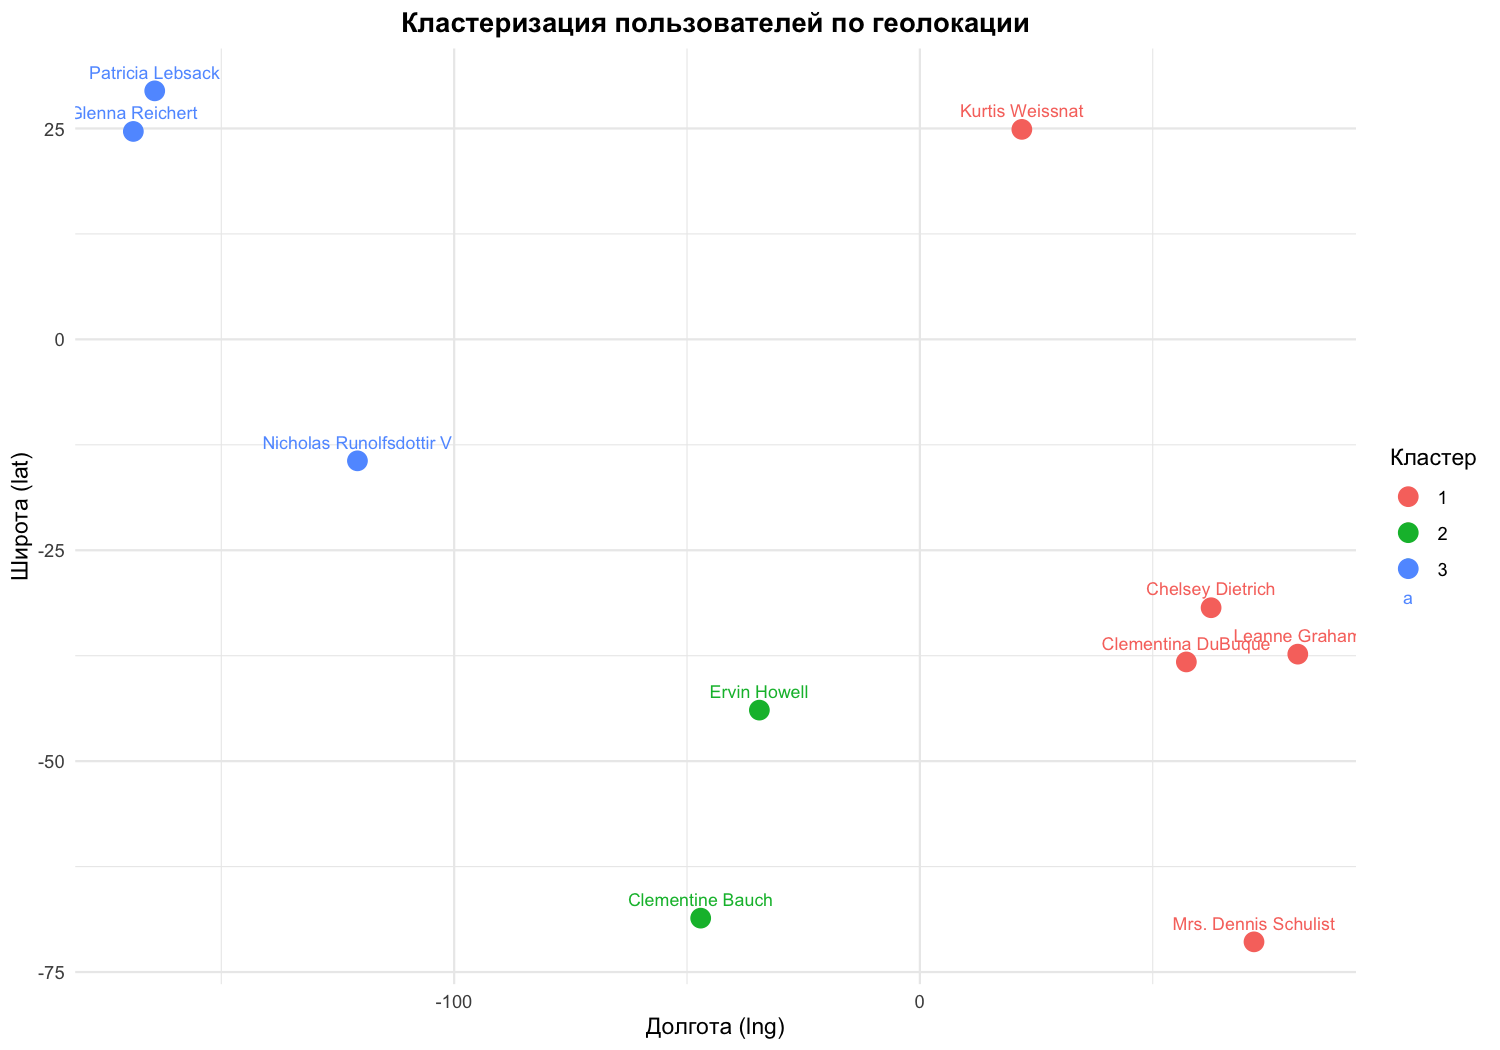
\includegraphics[width=0.85\textwidth]{cluster_scatter.png}
  \caption{Диаграмма рассеяния: кластеризация пользователей по геолокации}
  \label{fig:scatter}
\end{figure}

\begin{figure}[H]
  \centering
  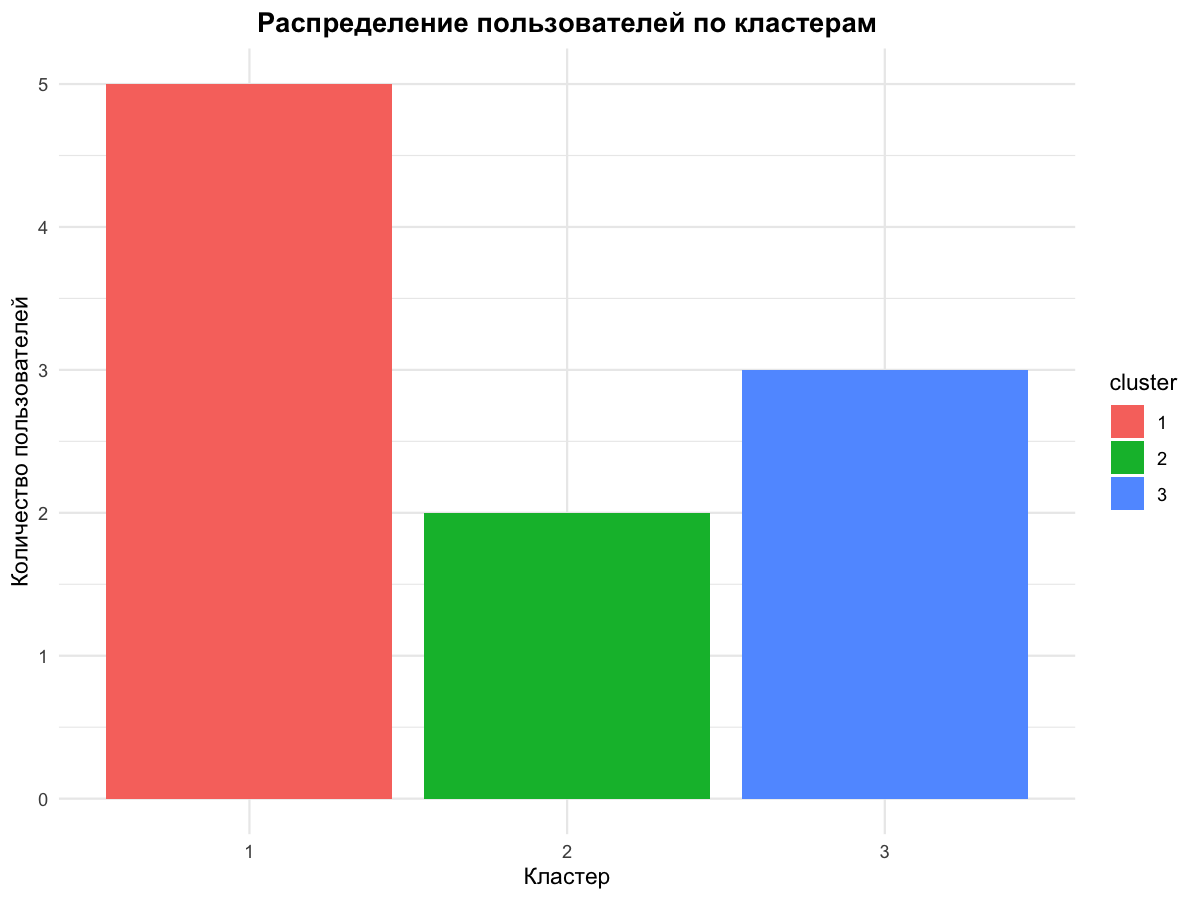
\includegraphics[width=0.7\textwidth]{cluster_bar.png}
  \caption{Столбиковая диаграмма распределения по кластерам}
  \label{fig:bar}
\end{figure}

\newpage

% =========================================================
% ЗАКЛЮЧЕНИЕ
% =========================================================
\addcontentsline{toc}{section}{Заключение}
\section*{ЗАКЛЮЧЕНИЕ}

В ходе выполнения лабораторной работы были получены следующие результаты:

1 Реализовано подключение к удалённому REST API (JSONPlaceholder) с использованием библиотеки httr и загрузка данных в формате JSON.

2 Данные о пользователях успешно извлечены, преобразованы в табличный формат и сохранены в локальный CSV-файл.

3 Проведён кластерный анализ методом k-средних по географическим координатам пользователей, выделено три кластера.

4 Результаты анализа визуализированы с помощью библиотеки ggplot2: построена диаграмма рассеяния с цветовой маркировкой кластеров и столбиковая диаграмма распределения.

5 Графические результаты сохранены в файлы формата PNG.

\newpage

% =========================================================
% СПИСОК ИСПОЛЬЗОВАННЫХ ИСТОЧНИКОВ
% =========================================================
\addcontentsline{toc}{section}{Список использованных источников}
\section*{СПИСОК ИСПОЛЬЗОВАННЫХ ИСТОЧНИКОВ}

\begin{enumerate}[label=\arabic*,leftmargin=1.25cm]
  \item The Comprehensive R Archive Network [Электронный ресурс].~-- Режим доступа: \url{https://cran.r-project.org/}.~-- Дата доступа: 10.04.2026.
  \item JSONPlaceholder~-- Free Fake REST API [Электронный ресурс].~-- Режим доступа: \url{https://jsonplaceholder.typicode.com/}.~-- Дата доступа: 10.04.2026.
  \item Wickham,~H. ggplot2: Elegant Graphics for Data Analysis / H.~Wickham.~-- 2nd ed.~-- New York~: Springer, 2016.~-- 260~p.
  \item Wickham,~H. R for Data Science / H.~Wickham, G.~Grolemund.~-- Sebastopol~: O'Reilly Media, 2017.~-- 492~p.
  \item Шипунов, А.\,Б. Анализ данных с R / А.\,Б.~Шипунов, А.\,И.~Коробейников, Е.\,М.~Балдин [Электронный ресурс].~-- Режим доступа: \url{https://inp.nsk.su/~baldin/DataAnalysis/R/R-07-datamining.pdf}.~-- Дата доступа: 10.04.2026.
  \item httr: Tools for Working with URLs and HTTP [Электронный ресурс].~-- Режим доступа: \url{https://httr.r-lib.org/}.~-- Дата доступа: 10.04.2026.
\end{enumerate}

\end{document}
